\documentclass[final,hyperref={pdfpagelabels=false}]{beamer}
\usepackage{grffile}
\mode<presentation>{\usetheme{byu}}
\usepackage[english]{babel}
\usepackage[latin1]{inputenc}
\usepackage{amsmath,amsthm, amssymb, latexsym}
\boldmath
\usepackage[orientation=landscape,size=a0,scale=1.5]{beamerposter}
\usepackage{array,booktabs,tabularx}
\newcolumntype{Z}{>{\centering\arraybackslash}X} \listfiles
\graphicspath{{figures/}}
\title{\huge Firefly Assembler: Parallelizing the Assembly of Genome Fragments}
\author{Kyle Corbitt, Dan Haskin}
\institute[Brigham Young University]{Molecular Biology and Computer Science Departments}
\date[Nov. 20th, 2013]{Nov. 20th, 2013}
\newlength{\columnheight}
\setlength{\columnheight}{105cm}
\begin{document}
\begin{frame}
    \begin{columns}
        \begin{column}{.32\textwidth}
            \begin{beamercolorbox}[center,wd=\textwidth]{postercolumn}
                \begin{minipage}[T]{.95\textwidth}
                    \parbox[t][\columnheight]{\textwidth}{
                        \begin{block}{Purpose}
                            By modeling genome assembly as a Travelling
                            Salesman Problem (TSP), we show how established
                            algorithms for getting near-optimal results on that
                            problem can be used for the purpose of solving the
                            genome assembly problem. One such algorithm is called
                            the Firefly algorithm (1).  This algorithm can
                            be paralellized and has been often used to solve
                            TSP with good results.
                        \end{block}
                        \begin{block}{Graph Representation}
                            In order to apply the LocalSearch and Firefly
                            algorithms to an assembly task we must first
                            represent the assembly as a graph.  An intuitive
                            method of accomplishing this is shown below.
                            \begin{center}
                                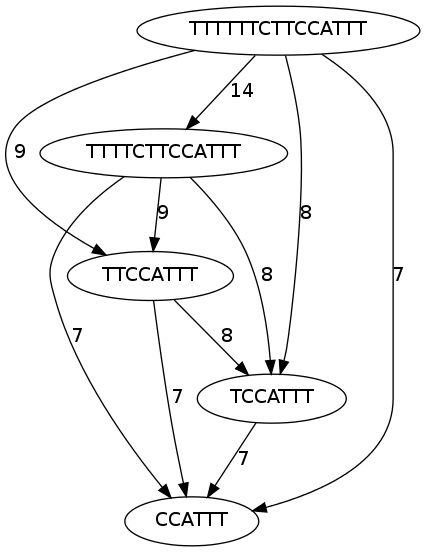
\includegraphics[scale=0.75]{example_graph}
                            \end{center}
                       \end{block}
                        \begin{block}{Greedy Algorithm}
                            As a base line, we use the greedy algorithm to
                            traverse the sequence overlap graph.  In essence,
                            the greatest overlaps are added to the path through
                            the graph first, followed by subsequent overlaps
                            added later to complete the path through the graph,
                            in order from greatest overlap to least.  This
                            algorithm is similar or equivalent to the
                            conventional shotgun sequencing technique used in
                            many sequence assemblers today.
                        \end{block}
                        \begin{block}{LocalSearch Algorithm}
                            As another comparison, we include the LocalSearch
                            algorithm in our results, which works by taking an
                            initial sequencing and then trying different small
                            variations on it to find a "better" graph traversal
                            (a longer traversal through the overlap graph).
                        \end{block}
                } \end{minipage}
            \end{beamercolorbox}
        \end{column}
        \begin{column}{.32\textwidth}
            \begin{beamercolorbox}[center,wd=\textwidth]{postercolumn}
                \begin{minipage}[T]{.95\textwidth}
                    \parbox[t][\columnheight]{\textwidth}{
                        \begin{block}{Firefly Algorithm}
                            In the firefly algorithm, A number of
                            random paths through the graph are generated, and
                            each one is called a "firefly". The algorithm
                            starts "moving" the fireflies (changing the paths)
                            toward other fireflies based on how "bright" (good)
                            they are, and how "close" (similar) they are to
                            each other, as shown below.
                            \begin{center}
                                \includegraphics[scale=1.0]{example_firefly}
                            \end{center}
                            {\em {\small photo courtesy of \url{http://www.mathworks.com/matlabcentral/fx_files/38931/3/SwarmFireFly_distance.jpg}. } }
                        \end{block}
                        \begin{block}{Methods}
                            We ran our algorithms against simulated reads
                            generated from scaffolds between 500 and 5000 base
                            pairs long with {\bf 5x} coverage and a median read
                            length of {\bf 100bp}. \\ \\
                            We measured the algorithms' performance on three
                            key metrics: the N50 length of the assemblies, the
                            total number of contigs found, and the time
                            necessary to run the algorithm.
                        \end{block}
                        \begin{block}{N50 comparison}
                            \begin{center}
                                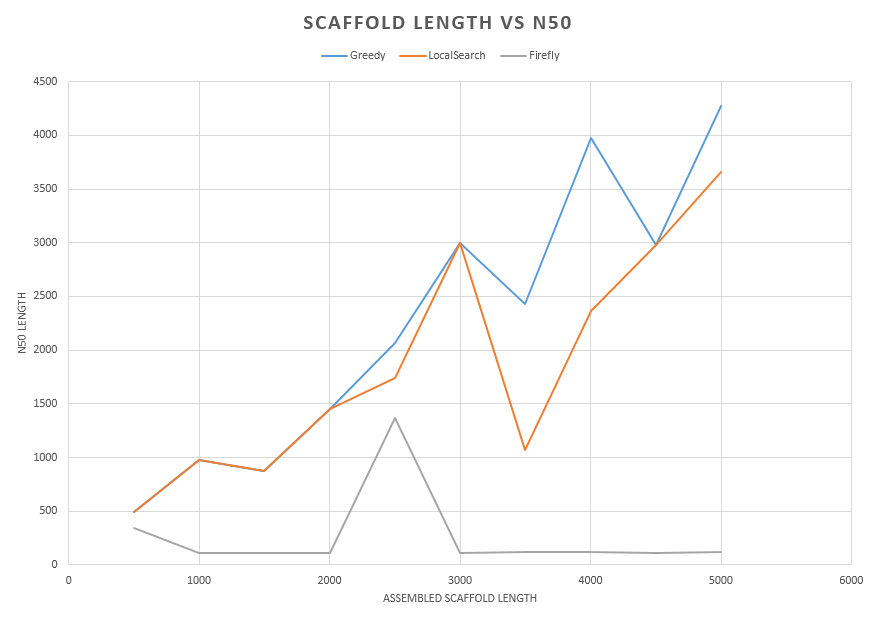
\includegraphics[scale=0.66]{n50}
                            \end{center}
                        \end{block}
                    }
        \end{minipage}
    \end{beamercolorbox}
        \end{column}
        \begin{column}{.32\textwidth}
            \begin{beamercolorbox}[center,wd=\textwidth]{postercolumn}
                \begin{minipage}[T]{.95\textwidth}
                    \parbox[t][\columnheight]{\textwidth}{
                        \begin{block}{Number of Contigs}
                            \begin{center}
                                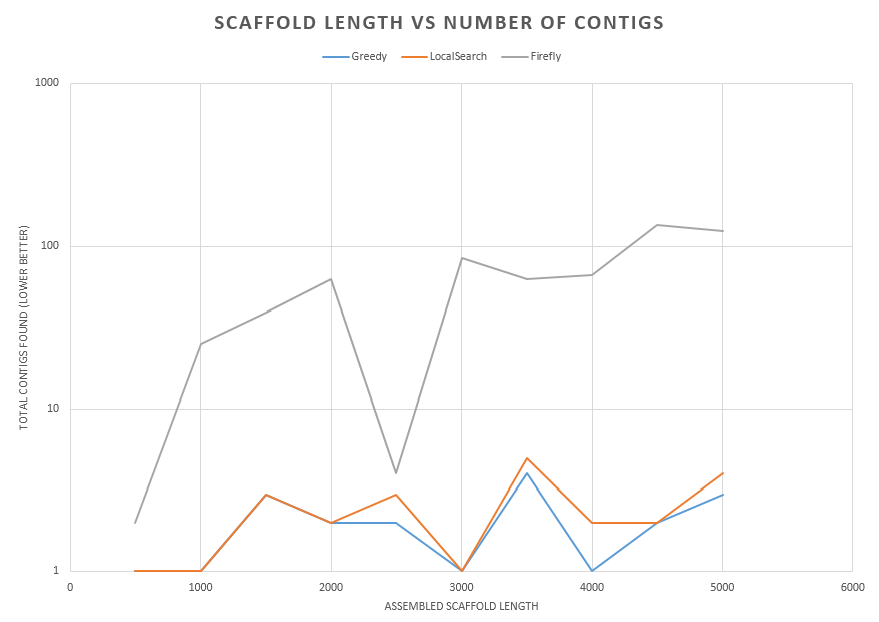
\includegraphics[scale=0.66]{num_contigs}
                            \end{center}
                        \end{block}
                        \begin{block}{Assembly Time}
                            \begin{center}
                                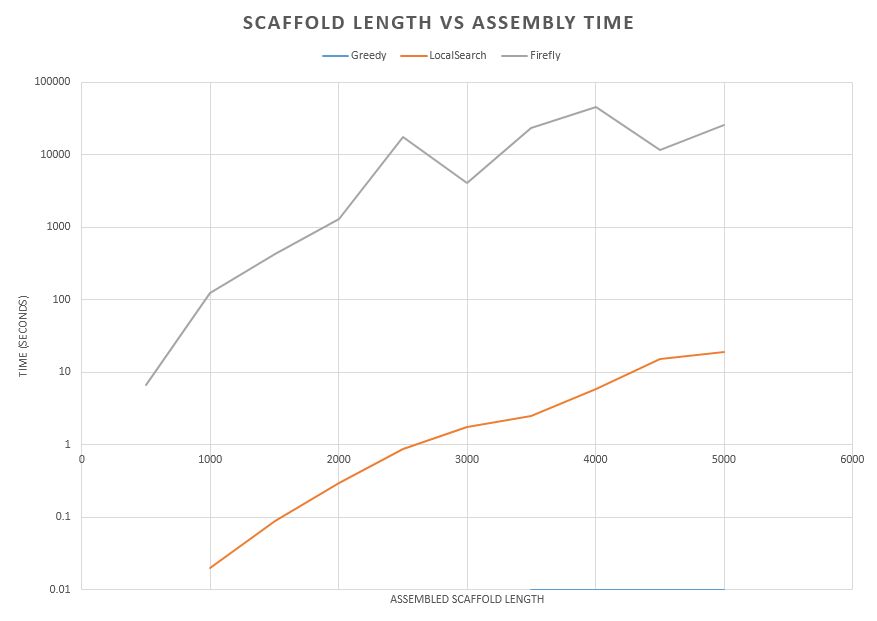
\includegraphics[scale=0.66]{assembly_time}
                            \end{center}
                        \end{block}
                        \begin{block}{Conclusions}
                            After reviewing our results, it is evident that our
                            implementation of the Firefly algorithm does not
                            perform well compared to greedy or local search,
                            even if it were to be parallelized. \\
                            \\
                            Somewhat surprsingly, we do find that local search
                            sometimes performs better than greedy in making
                            longer contigs; however, this algorithm is not
                            paralellizable.
                        \end{block}
                        \begin{block}{Literature}
                            {\tiny
                                \setbeamertemplate{bibliography item}[text]
                                \bibliographystyle{abbrv}
                                \nocite{*}
                                \bibliography{poster}
                            }
                        \end{block}
                    }
                \end{minipage}
            \end{beamercolorbox}
        \end{column}
    \end{columns}
    \vskip1ex
    \tiny\hfill{Created with \LaTeX \texttt{beamerposter}  \url{http://www-i6.informatik.rwth-aachen.de/~dreuw/latexbeamerposter.php} \hskip1em}
\end{frame}
\end{document}
